%%%%%%%%%%%%%%%%%%%%%%%%%%%%%%%%%%%%%%%%%
% Lachaise Assignment
% LaTeX Template
% Version 1.1(26/6/2018)
%
% This template originates from:
% http://www.LaTeXTemplates.com
%
% Authors:
% Marion Lachaise & François Févotte
% Vel (vel@LaTeXTemplates.com)
%
% License:
% CC BY-NC-SA 3.0 (http://creativecommons.org/licenses/by-nc-sa/3.0/)
% 
%%%%%%%%%%%%%%%%%%%%%%%%%%%%%%%%%%%%%%%%

%----------------------------------------------------------------------------------------
%	PACKAGES AND OTHER DOCUMENT CONFIGURATIONS
%----------------------------------------------------------------------------------------

\documentclass{article}

%%%%%%%%%%%%%%%%%%%%%%%%%%%%%%%%%%%%%%%%%
% Lachaise Assignment
% Structure Specification File
% Version 1.0 (26/6/2018)
%
% This template originates from:
% http://www.LaTeXTemplates.com
%
% Authors:
% Marion Lachaise & François Févotte
% Vel (vel@LaTeXTemplates.com)
%
% License:
% CC BY-NC-SA 3.0 (http://creativecommons.org/licenses/by-nc-sa/3.0/)
% 
%%%%%%%%%%%%%%%%%%%%%%%%%%%%%%%%%%%%%%%%%

%----------------------------------------------------------------------------------------
%	PACKAGES AND OTHER DOCUMENT CONFIGURATIONS
%----------------------------------------------------------------------------------------

\usepackage{amsmath,amsfonts,stmaryrd,amssymb,bbm,float,graphicx,enumerate,mathtools,listings,xcolor,color,esint,subfig,tikz,pgfplots,adjustbox,setspace,bm,minted,pdfpages,hyperref} % Math packages

\usepackage{enumerate} % Custom item numbers for enumerations

\usepackage[lined,boxed,vlined,ruled]{algorithm2e}
\SetKw{Continue}{continue}
\SetKw{Or}{or}
\SetKw{Until}{until}

\usepackage[framemethod=tikz]{mdframed} % Allows defining custom boxed/framed environments

\usepackage{listings} % File listings, with syntax highlighting
\lstset{
    basicstyle=\ttfamily, % Typeset listings in monospace font
}

\DeclarePairedDelimiter\ceil{\lceil}{\rceil}
\DeclarePairedDelimiter\floor{\lfloor}{\rfloor}

% Allow for the \begin{align} to go over the page
\allowdisplaybreaks

%----------------------------------------------------------------------------------------
%	DOCUMENT MARGINS
%----------------------------------------------------------------------------------------

\usepackage{geometry} % Required for adjusting page dimensions and margins

\geometry{
    paper=a4paper, % Paper size, change to letterpaper for US letter size
    top=2.5cm, % Top margin
    bottom=3cm, % Bottom margin
    left=2.5cm, % Left margin
    right=2.5cm, % Right margin
    headheight=14pt, % Header height
    footskip=1.5cm, % Space from the bottom margin to the baseline of the footer
    headsep=1.2cm, % Space from the top margin to the baseline of the header
    %showframe, % Uncomment to show how the type block is set on the page
}

%----------------------------------------------------------------------------------------
%	FONTS
%----------------------------------------------------------------------------------------

\usepackage[utf8]{inputenc} % Required for inputting international characters
\usepackage[T1]{fontenc} % Output font encoding for international characters

\usepackage{XCharter} % Use the XCharter fonts

%----------------------------------------------------------------------------------------
%	COMMAND LINE ENVIRONMENT
%----------------------------------------------------------------------------------------

% Usage:
% \begin{commandline}
%	\begin{verbatim}
%		$ ls
%		
%		Applications	Desktop	...
%	\end{verbatim}
% \end{commandline}

\mdfdefinestyle{commandline}{
    leftmargin=10pt,
    rightmargin=10pt,
    innerleftmargin=15pt,
    middlelinecolor=black!50!white,
    middlelinewidth=2pt,
    frametitlerule=false,
    backgroundcolor=black!5!white,
    frametitle={Command Line},
    frametitlefont={\normalfont\sffamily\color{white}\hspace{-1em}},
    frametitlebackgroundcolor=black!50!white,
    nobreak,
}

% Define a custom environment for command-line snapshots
\newenvironment{commandline}{
    \medskip
    \begin{mdframed}[style=commandline]
        }{
    \end{mdframed}
    \medskip
}

%----------------------------------------------------------------------------------------
%	FILE CONTENTS ENVIRONMENT
%----------------------------------------------------------------------------------------

% Usage:
% \begin{file}[optional filename, defaults to "File"]
%	File contents, for example, with a listings environment
% \end{file}

\mdfdefinestyle{file}{
    innertopmargin=1.6\baselineskip,
    innerbottommargin=0.8\baselineskip,
    topline=false, bottomline=false,
    leftline=false, rightline=false,
    leftmargin=2cm,
    rightmargin=2cm,
    singleextra={%
            \draw[fill=black!10!white](P)++(0,-1.2em)rectangle(P-|O);
            \node[anchor=north west]
            at(P-|O){\ttfamily\mdfilename};
            %
            \def\l{3em}
            \draw(O-|P)++(-\l,0)--++(\l,\l)--(P)--(P-|O)--(O)--cycle;
            \draw(O-|P)++(-\l,0)--++(0,\l)--++(\l,0);
        },
    nobreak,
}

% Define a custom environment for file contents
\newenvironment{file}[1][File]{ % Set the default filename to "File"
    \medskip
    \newcommand{\mdfilename}{#1}
    \begin{mdframed}[style=file]
        }{
    \end{mdframed}
    \medskip
}

%----------------------------------------------------------------------------------------
%	NUMBERED QUESTIONS ENVIRONMENT
%----------------------------------------------------------------------------------------

% Usage:
% \begin{question}[optional title]
%	Question contents
% \end{question}

\mdfdefinestyle{question}{
    innertopmargin=1.2\baselineskip,
    innerbottommargin=0.8\baselineskip,
    roundcorner=5pt,
    nobreak,
    singleextra={%
            \draw(P-|O)node[xshift=1em,anchor=west,fill=white,draw,rounded corners=5pt]{%
                Question \theQuestion\questionTitle};
        },
}

\newcounter{Question} % Stores the current question number that gets iterated with each new question

% Define a custom environment for numbered questions
\newenvironment{question}[1][\unskip]{
    \bigskip
    \stepcounter{Question}
    \newcommand{\questionTitle}{~#1}
    \begin{mdframed}[style=question]
        }{
    \end{mdframed}
    \medskip
}

%----------------------------------------------------------------------------------------
%	WARNING TEXT ENVIRONMENT
%----------------------------------------------------------------------------------------

% Usage:
% \begin{warn}[optional title, defaults to "Warning:"]
%	Contents
% \end{warn}

\mdfdefinestyle{warning}{
    topline=false, bottomline=false,
    leftline=false, rightline=false,
    nobreak,
    singleextra={%
            \draw(P-|O)++(-0.5em,0)node(tmp1){};
            \draw(P-|O)++(0.5em,0)node(tmp2){};
            \fill[black,rotate around={45:(P-|O)}](tmp1)rectangle(tmp2);
            \node at(P-|O){\color{white}\scriptsize\bf !};
            \draw[very thick](P-|O)++(0,-1em)--(O);%--(O-|P);
        }
}

% Define a custom environment for warning text
\newenvironment{warn}[1][Warning:]{ % Set the default warning to "Warning:"
    \medskip
    \begin{mdframed}[style=warning]
        \noindent{\textbf{#1}}
        }{
    \end{mdframed}
}

%----------------------------------------------------------------------------------------
%	INFORMATION ENVIRONMENT
%----------------------------------------------------------------------------------------

% Usage:
% \begin{info}[optional title, defaults to "Info:"]
% 	contents
% 	\end{info}

\mdfdefinestyle{info}{%
topline=false, bottomline=false,
leftline=false, rightline=false,
nobreak,
singleextra={%
\fill[black](P-|O)circle[radius=0.4em];
\node at(P-|O){\color{white}\scriptsize\bf i};
\draw[very thick](P-|O)++(0,-0.8em)--(O);%--(O-|P);
}
}

% Define a custom environment for information
\newenvironment{info}[1][Info:]{ % Set the default title to "Info:"
    \medskip
    \begin{mdframed}[style=info]
        \noindent{\textbf{#1}}
        }{
    \end{mdframed}
}

\pgfplotsset{compat=1.12}
\usepgfplotslibrary{fillbetween}
\DeclareMathOperator{\sech}{sech}
\DeclareMathOperator{\arcsech}{arcsech}
\DeclareMathOperator{\arcoth}{arcoth}
\DeclareMathOperator{\arctanh}{tanh^{-1}}
\renewcommand{\baselinestretch}{1.25}
\newcommand{\bin}{{\sf Bin}}
\newcommand{\G}{{\sf G}}
\newcommand{\Hyp}{{\sf Hyp}}
\newcommand{\Ber}{{\sf Ber}}
\newcommand{\Po}{{\sf Po}}
\newcommand{\Poi}{{\sf Poi}}
\newcommand{\ex}{{\sf Exp}}
\newcommand{\Nor}{{\sf N}}
\newcommand{\gam}{{\sf Gam}}
\newcommand{\Em}{\mathbb E}
\newcommand{\Pm}{\mathbb P}
\newcommand{\R}{\mathbb R}
\newcommand{\Cm}{\mathbb C}
\newcommand{\B}{\cal B}
\newcommand{\F}{\mathbb F}
\newcommand{\N}{\mathbb N}
\newcommand{\Z}{\mathbb Z}
\newcommand{\Q}{\mathbb Q}
\newcommand{\Comp}{\mathbb C}
\newcommand{\e}{\mbox{e}}
\newcommand{\Var}{\mbox{Var}}
\newcommand{\cov}{\mbox{Cov}}
\newcommand{\ds}{\displaystyle}
\newcommand{\subvect}[1]{\mbox{\small \boldmath #1}}
%\newcommand{\vect}[1]{\mbox{\boldmath $#1$}}
\newcommand{\vect}[1]{\boldsymbol #1}
\newcommand{\norm}[1]{\left\lVert#1\right\rVert}
\newcommand*\VF[1]{\mathbf{#1}}
\newcommand*\dif{\mathop{}\!\mathrm{d}}
\setlength{\jot}{7pt}
\definecolor{lbcolor}{rgb}{0.95,0.95,0.95}

\title{COMP4702: 2021 Final Exam} % Title of the assignment

\author{Michael Ciccotosto-Camp\\ \texttt{s4430291}} % Author name and email address

\date{University of Queensland --- \today}
\begin{document}

\maketitle % Print the title

\section*{Data Edits and Visualizations}

% \begin{itemize}
%     \item What changes where made to the dataset. Were rows/columns removed or edited? Why?
%     \item What any standardization/normalization performed?
%     \item Does the data look easy to separate when projected onto a lower dimension using PCA,TSNE, etc? How might this influence which model we use?
%     \item Graph the covariances between the data.
% \end{itemize}

To start rows that contained Nan values where removed from the data set so that all the features could be utilized for prediction. It was decided that we could try turning this into a classification problem by predicting the last column (with two classes, "b" and "g") a using the remaining as inputs. The last column was encoded to integer values using sklearns \texttt{LabelEncoder} function. Remaining columns where standardized using sklearns \texttt{StandardScaler} function. The distribution of classes is shown below.

\begin{figure}[H]
    \centering
    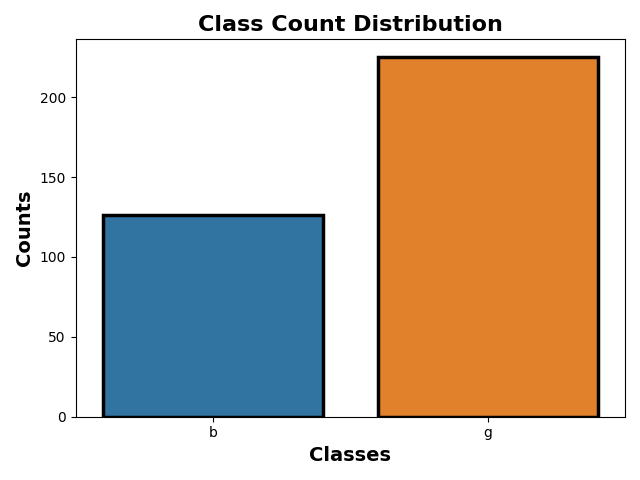
\includegraphics[scale=0.5]{cls_dist.png}
    \caption{Class distribution}
\end{figure}

A SCREE graph and covariance matrix was also produced for this data set.

\begin{figure}[H]
    \centering
    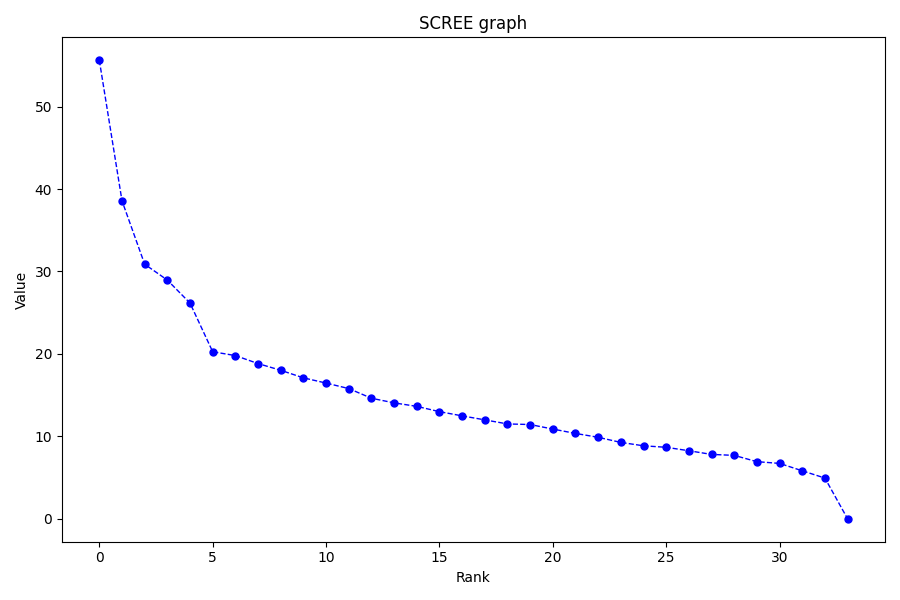
\includegraphics[scale=0.5]{scree_plot.png}
    \caption{SCREE graph}
\end{figure}

\begin{figure}[H]
    \centering
    
\includegraphics[scale=0.4]{cov_mat.png}
    \caption{Covariance Matrix}
\end{figure}

One thing to notice is that the vast majority of importance weighting in the spree graph resides in the first 5 principal components. This suggests that the data undergo dimensionality reduction without too much feature information loss. This is supported by the fact that there are a number of correlations depicted in the covariance matrix. A number of dimensionality reduction techniques were used project the data onto a 2-dimensional to see how well they separate out the data. Each feature was standardized before hand so that the dimensionality reduction techniques so that no feature had a information retention weighting. The techniques used were PCA, TSNE. The results are presented below.

\begin{figure}[H]
    \centering
    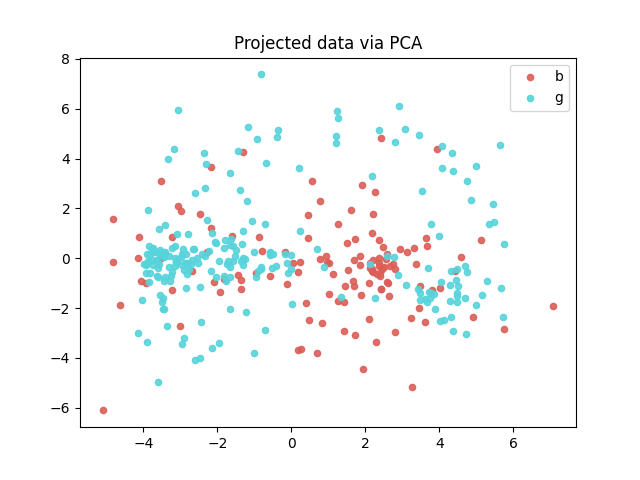
\includegraphics[scale=0.7]{projection_PCA.png}
\end{figure}

\begin{figure}[H]
    \centering
    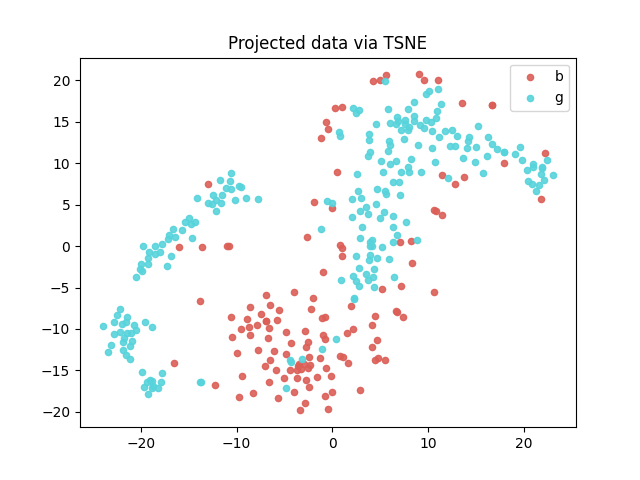
\includegraphics[scale=0.7]{projection_TSNE.png}
\end{figure}

\begin{figure}[H]
    \centering
    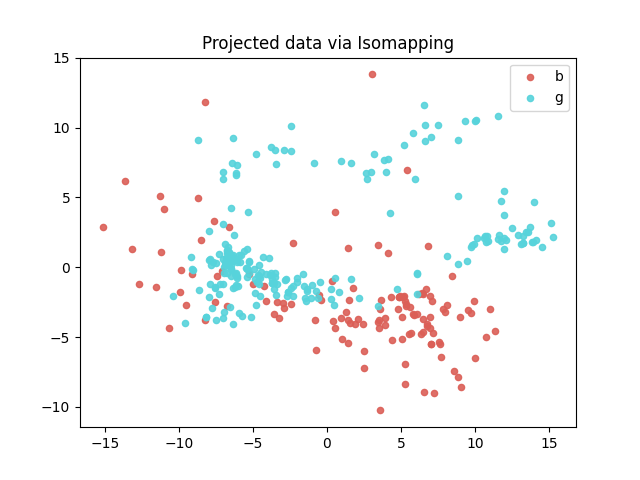
\includegraphics[scale=0.7]{projection_ISO.png}
\end{figure}

% \begin{figure}[H]
%     \centering
%     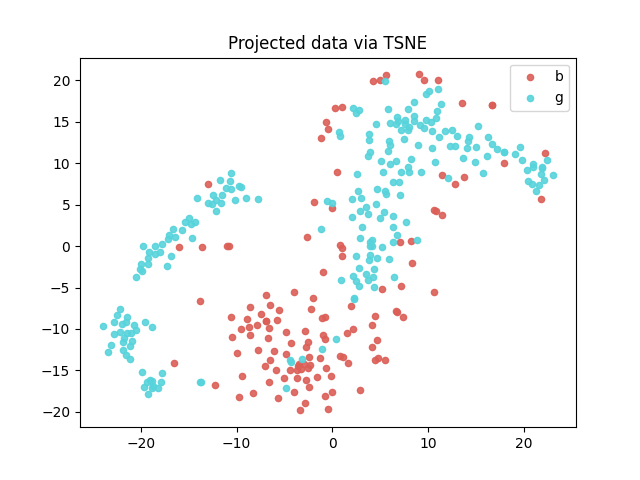
\includegraphics[scale=0.7]{projection_TSNE.png}
% \end{figure}

TSNE was chosen to be the preferred method for dimensionality reduction since it seemed to provide the best separation between classes.

\section*{Logistic Regression Model}

% \begin{itemize}
%     \item What model was chosen? Explain why the selected model is suitable for the task at hand (eg its a good idea use SVC if a classification problem is given to us and all the inputs are continuous).
%     \item What parameters were selected? Were they adjusted/how?
% \end{itemize}

A Logistic Regression model was chosen since these models are designed to perform classification tasks on binary inputs. sklearn's \texttt{LogisticRegression} implementation was used for this. A grid search was used to find the best parameters for the regularization strength (C) and tolerance for stopping criteria (tol). To do this, numerous Logistic Regression model's were trained with various combinations of different values for C and tol and the performance of each model was measured by averaging the accuracy of a 5-fold cross validation partition. The results of the grid search are shown below.

\begin{figure}[H]
    \centering
    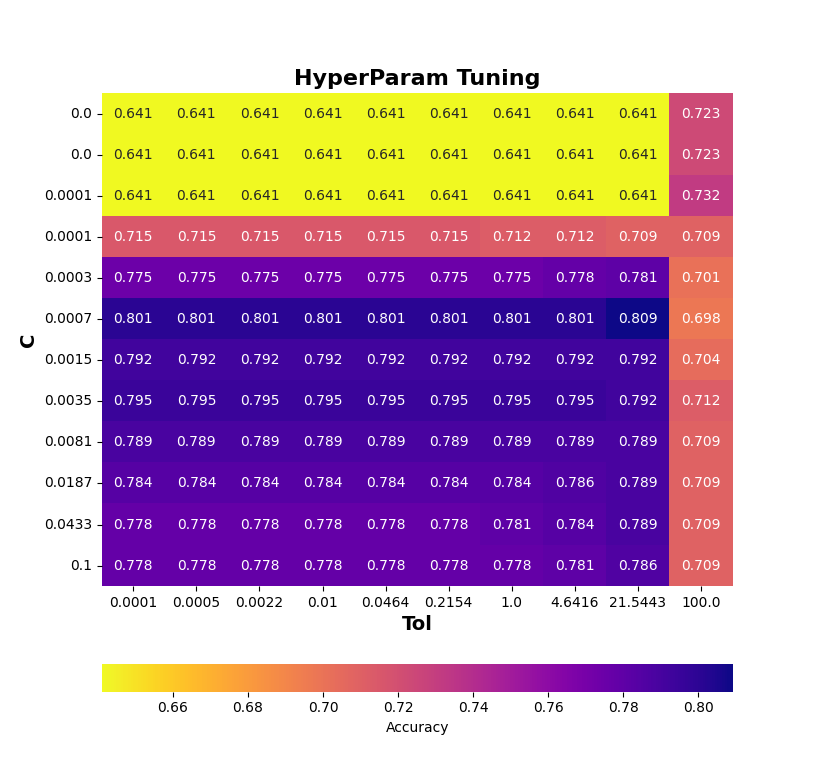
\includegraphics[scale=0.7]{lg_param_tune.png}
\end{figure}

Thus the parameters for this model was set to $C=0.809, tol=21.5443$ as the yielded the best cross validation scores. A confusion matrix and a visualizations of model predictions is shown below for a typical run when $1/5$ of the dataset is reversed for testing. Again, the data is projected onto a 2-dimensional plane via TSNE.

\begin{figure}[H]
    \centering
    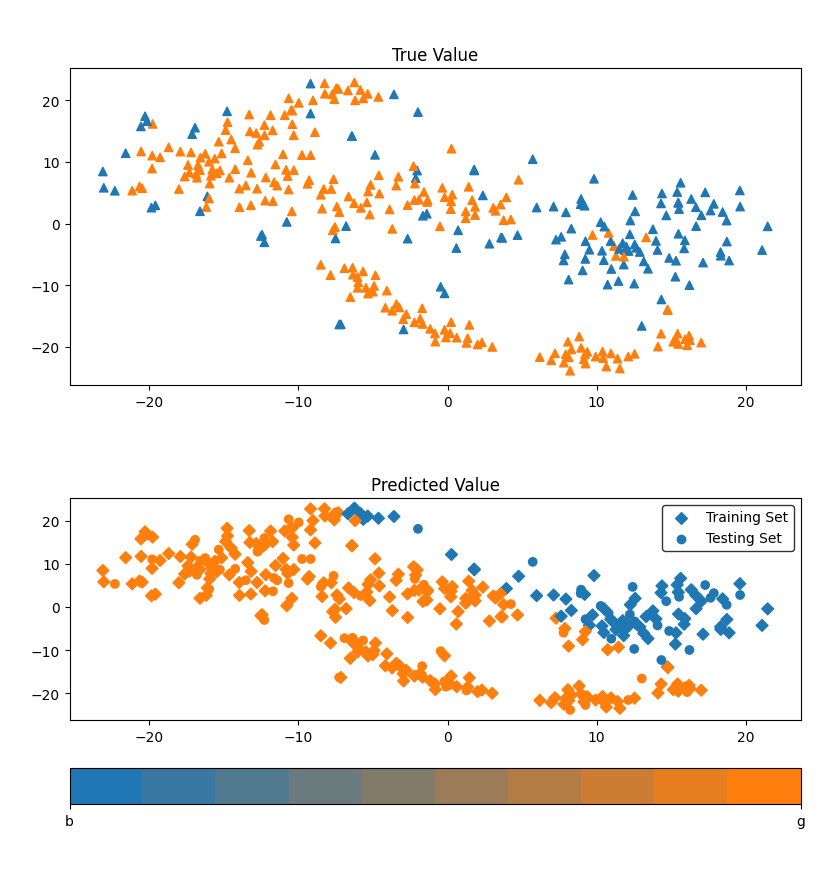
\includegraphics[scale=0.7]{true_vs_pred_lg.png}
\end{figure}

\begin{figure}[H]
    \centering
    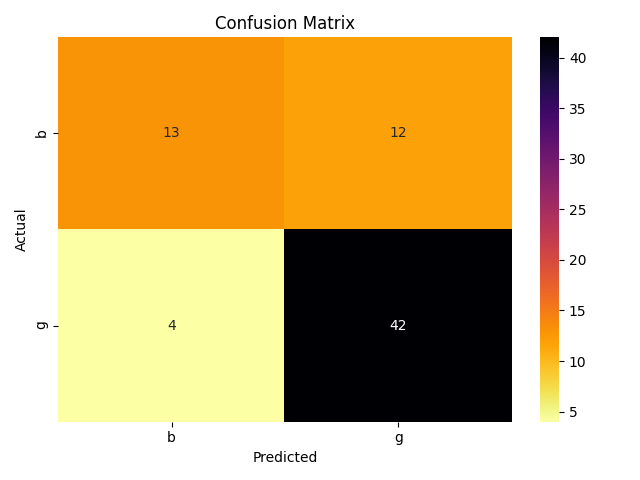
\includegraphics[scale=0.7]{conf_mat.png}
\end{figure}

We can see that the model does poorly to distinguish between inputs when there is a lot of overlap between classes since they only make one partition in the dataset. We can also see there are many more missclassification with values from the "b" class (being incorrectly labeled as an input from "g") as a result of the boundary trying to maximise correct classification for the "g" as the are far more of them.

\section*{Neural Network Model}

A neural network model was also used since, although TSNE provides a good separation of classes in lower dimensions, there is still small amount of class overlap causing models using data reduced via TSNE to occasional misclassify points. The complexity of a neural network architecture may mean it could learn a non-trivial way to separate and classify points. To this end, an initial neural network architecture of a single hidden layer with relu activation and a single output with a sigmoid activation function was devised. The 6-layer hidden layer adds extra complexity to the model to assist in learning highly non-trivial and non-linear functions which one can also think of as also providing some sort of in-built dimensionality reduction. Relu activation functions were used for efficiently and are well known for generally providing good performance. A sigmoid function was used to turn the output into a value ranging between 0 and 1 (which can be interpreted as a probability of belonging to a class of 1). An Adam optimizer was used as it combines RMSProp with standard momentum meaning it generally has better learning rate adaptation than most other optimizers such as Adagrad, RMSProp and AdaDelta. Binary cross entropy was used as the loss function as it minimizes the dissimilarity between the empirical distribution of training data and the the distribution induced by the model for binary classification problems and directly optimizes the cross-entropy leading to naturally well-calibrated probabilities. A grid search over the learning rates was done to determine which learning rates was optimal for model training. The performance of each learning rates was measured by averaging the accuracy of a 5-fold cross validation partition. The model accuracies using different learning rates and an epoch of 50 is graphed below.

From the graph learning rates between ... and ... provided the best results and a learning rate of ... was choosen for the remainder of experimentation. The validation and training loss was graphed over the number of epochs to see were overfitting may occur.

\begin{figure}[H]
    \centering
    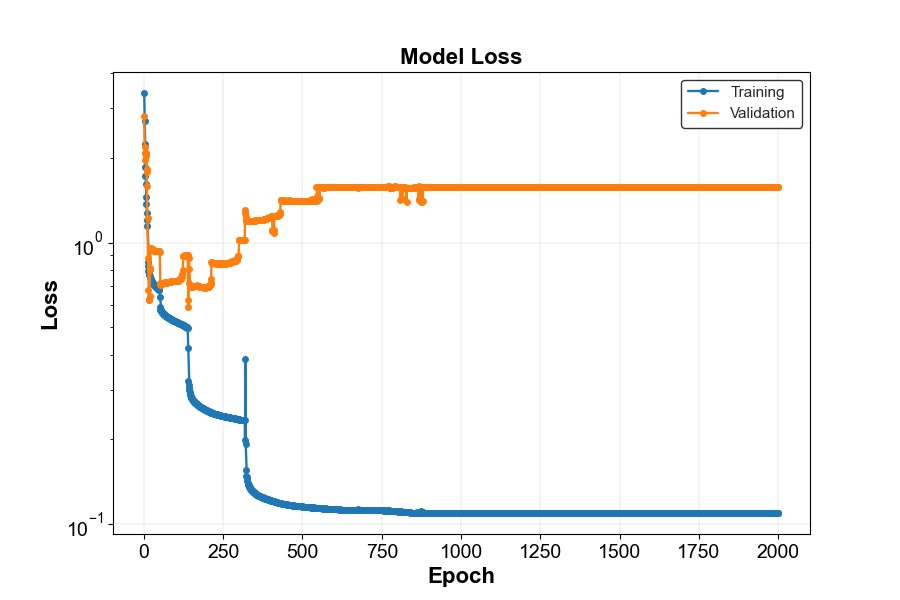
\includegraphics[scale=0.7]{nn_model_loss.png}
\end{figure}

As we can see, training the model beyond 100 epochs is likely going to overfit our model. Thus, the model was only trained with 100 epochs for the remainder of experimentation. A confusion matrix and a visualizations of model predictions is shown below for a typical run when $1/5$ of the dataset is reversed for testing. The data is projected onto a 2-dimensional plane via TSNE (but note that TSNE is not used anywhere within the prediction process).

\begin{figure}[H]
    \centering
    
\includegraphics[scale=0.7]{true_vs_pred_nn.png}
\end{figure}

\begin{figure}[H]
    \centering
    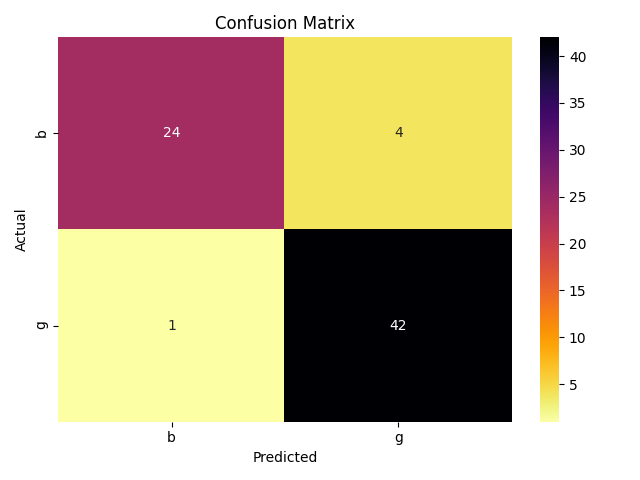
\includegraphics[scale=0.7]{conf_mat_nn.png}
\end{figure}

The training and testing errors had also been recorded over $10$ runs where accuracies where measured by averaging the accuracy of a 5-fold cross validation partition.

\begin{table}[h!]
    \centering
    \begin{tabular}{rrr}
        \hline
        Repetition & Train Acc & Test Acc \\
        \hline
        0          & 0.99715   & 0.957626 \\
        1          & 1         & 0.997143 \\
        2          & 1         & 1        \\
        3          & 1         & 1        \\
        4          & 1         & 1        \\
        5          & 1         & 1        \\
        6          & 1         & 1        \\
        7          & 1         & 1        \\
        8          & 1         & 1        \\
        9          & 1         & 1        \\
        \hline
    \end{tabular}
\end{table}

It is very obvious that the neural network model performes far better when the Logistic Regression model as it is no longer restricted to a partition line within the feature space, but can learn a far more intricate separation boundary, pressumably in a higher dimensional space. As a result, we find it correctly identities far more inputs as belonging to the "b" classes.

\begin{minted}[mathescape,
    linenos,
    numbersep=5pt,
    frame=lines,
    framesep=2mm]{python}
    #!/usr/bin/env python3

    __author__ = 'Michael Ciccotosto-Camp'
    __version__ = ''
    
    import os
    from sklearn.metrics import accuracy_score, mean_squared_error
    import torch
    import pandas as pd
    import numpy as np
    import seaborn as sns
    import matplotlib as mpl
    import matplotlib.pyplot as plt
    
    from sklearn.decomposition import PCA
    
    
    def drop_high_nan(df, prop=0.2):
        """
        Drops columns from a dataframe with a high proportion of Nan values.
    
        Parameters:
            df:
                A pandas Dataframe which we would like to clean.
    
            prop:
                The the threshold proportion to drop a row from the df.
        """
        n, _ = df.shape
        to_drop = []
    
        for col in df.columns:
            num_nans = (df[col]).isna().sum()
            if num_nans / n > prop:
                to_drop.append(col)
    
        df.drop(columns=to_drop, inplace=True)
        return
    
    
    def plot_cls_dist(y, labels):
        """
        Counts the number of occurrences of each class.
        """
        y_counts = np.bincount(y)
        df = {
            "Classes": labels,
            "Counts": y_counts,
        }
        df = pd.DataFrame(df)
        ax = sns.barplot(x="Classes", y="Counts", data=df, capsize=.1,
                         linewidth=2.5, ci=None, edgecolor="black", fill=True)
        ax.set_title("Class Count Distribution", fontsize=16, fontweight="bold")
        ax.set_xlabel("Classes", fontsize=14, fontweight="bold")
        ax.set_ylabel("Counts", fontsize=14, fontweight="bold")
        plt.tight_layout()
        plt.show()
        # plt.savefig(os.path.join(save_dir, settings["save_name"]))
        plt.cla()
        plt.clf()
    
        return
    
    
    def true_vs_pred(X, y, X_train, y_train_pred, X_test, y_test_pred, reg=True, save_path=None, classes=None):
        """
        Graphs true values of y along side predictions.
    
        Parameters:
            X:
                A 2-row numpy representation of the entire dataset.
            y:
                A numpy vector of true outputs.
            X_train:
                A 2-row numpy representation of the training data.
            y_train_pred:
                A numpy vector contain predictions for the testing dataset.
            X_test:
                A 2-row numpy representation of the testing data.
            y_test_pred:
                A numpy vector contain predictions for the testing dataset.
            reg:
                Keep true if this was a regression task, set to false otherwise.
            classes:
                A list or ordered classess for regression.
        """
    
        fig = plt.figure()
        if reg:
            vmin, vmax = np.min(y), np.max(y)
            ax = fig.add_subplot(211)
            ax.set_title("True Value")
            ax.scatter(X[:, 0], X[:, 1], c=y,
                       cmap=plt.cm.Spectral, vmin=vmin, vmax=vmax, marker="^")
    
            ax = fig.add_subplot(212)
            ax.set_title("Predicted Value")
            ax.scatter(X_train[:, 0], X_train[:, 1], c=y_train_pred,
                       cmap=plt.cm.Spectral, vmin=vmin, vmax=vmax,
                       marker="D")
            im = ax.scatter(X_test[:, 0], X_test[:, 1], c=y_test_pred,
                            cmap=plt.cm.Spectral, vmin=vmin, vmax=vmax,
                            marker="o")
            plt.legend(["Training Set", "TestingSet"], edgecolor="black")
            plt.colorbar(im, orientation="horizontal")
        else:
            vmin, vmax = int(np.min(y)), int(np.max(y))
            n = np.unique(y)
            cmap = plt.cm.tab10
            # extract all colors from the .jet map
            cmaplist = [cmap(i) for i in n]
            # create the new map
            cmap = mpl.colors.LinearSegmentedColormap.from_list(
                'Custom cmap', cmaplist, cmap.N)
            ax = fig.add_subplot(211)
            ax.set_title("True Value")
            ax.scatter(X[:, 0], X[:, 1], c=y,
                       cmap=cmap, vmin=vmin, vmax=vmax, marker="^")
    
            ax = fig.add_subplot(212)
            ax.set_title("Predicted Value")
            ax.scatter(X_train[:, 0], X_train[:, 1], c=y_train_pred,
                       cmap=cmap, vmin=vmin, vmax=vmax,
                       marker="D")
            im = ax.scatter(X_test[:, 0], X_test[:, 1], c=y_test_pred,
                            cmap=cmap, vmin=vmin, vmax=vmax,
                            marker="o")
            plt.legend(["Training Set", "Testing Set"], edgecolor="black")
            cb = plt.colorbar(im, spacing='proportional', orientation="horizontal")
            loc = np.arange(0, vmax + 1, 1)
            cb.set_ticks(loc)
            cb.set_ticklabels(classes)
        plt.tight_layout()
        if save_path is not None:
            plt.savefig(save_path)
        else:
            plt.show()
        plt.cla()
        plt.clf()
    
        return
    
    
    def CV_heatmap_sklearn(model, X, y, feat_1, feat_2, feat_1_range, feat_2_range, m_args=tuple(), m_kwargs={}):
        """
        Produces a heat map for gridsearching along various hyperparameters. Using
        CV.
    
        Parameters:
            model:
                A callable to create an instance of the desired model, eg svm.SVC.
            X:
                A numpy matrix containing input vectors.
            y:
                A numpy array containing output vectors.
            feat_1:
                The name of the first feature to search for as a string, eg the 
                "gamma" for the svm.SVC model.
            feat_2:
                The name of the second feature to search for as a string.
            feat_1_range:
                The range of (iterable) values to search over for the first 
                feature, eg [1e-1,1e-0,1e1].
            feat_2_range:
                The range of (iterable) values to search over for the second feature.
        """
        from sklearn.model_selection import cross_val_score
        acc = np.empty((len(feat_1_range), len(feat_2_range)))
    
        for f1i, feat_1_val in enumerate(feat_1_range):
            for f2i, feat_2_val in enumerate(feat_2_range):
                m_kwargs[feat_1] = feat_1_val
                m_kwargs[feat_2] = feat_2_val
                clf = model(*m_args, **m_kwargs)
                scores = cross_val_score(clf, X, y, cv=5)
                acc[f1i, f2i] = np.mean(scores)
    
        grid_kws = {"height_ratios": (.9, .05), "hspace": .3}
        f, (ax, cbar_ax) = plt.subplots(2, gridspec_kw=grid_kws)
        ax = sns.heatmap(np.abs(acc), ax=ax,
                         annot=True,
                         fmt='.3f',
                         cmap="plasma_r",
                         cbar_ax=cbar_ax,
                         cbar_kws={"orientation": "horizontal",
                         'label': 'Accuracy'})
        ax.set_title("HyperParam Tuning", fontsize=16, fontweight="bold")
        ax.set_xticklabels(
            list(map(lambda x: float("{:.4f}".format(x)), list(feat_2_range))))
        ax.set_yticklabels(
            list(map(lambda x: float("{:.4f}".format(x)), list(feat_1_range))),
            rotation=0, va="center")
        ax.set_xlabel(feat_2.title(), fontsize=14, fontweight="bold")
        ax.set_ylabel(feat_1.title(), fontsize=14, fontweight="bold")
        # plt.tight_layout()
        plt.show()
        plt.cla()
        plt.clf()
        return
    
    
    def CV_onevar_sklearn(model, X, y, feat, feat_range, m_args=tuple(), m_kwargs={}):
        """
        Produces a heat map for gridsearching along various hyperparameters. Using
        CV.
    
        Parameters:
            model:
                A callable to create an instance of the desired model, eg svm.SVC.
            X:
                A numpy matrix containing input vectors.
            y:
                A numpy array containing output vectors.
            feat:
                The name of the feature to search for as a string, eg the
                "gamma" for the svm.SVC model.
            feat_range:
                The range of (iterable) values to search over for the first
                feature, eg [1e-1,1e-0,1e1].
        """
        from sklearn.model_selection import cross_val_score
        acc = np.empty(len(feat_range))
    
        for f1i, feat_val in enumerate(feat_range):
            m_kwargs[feat] = feat_val
            clf = model(*m_args, **m_kwargs)
            scores = cross_val_score(clf, X, y, cv=5)
            acc[f1i] = np.mean(scores)
    
        plot_meteric([(feat_range.squeeze(), acc.squeeze(), feat)], f"CV on {feat}",
                     "Value", "Accuracy", log_x=True)
    
        # grid_kws = {"height_ratios": (.9, .05), "hspace": .3}
        # f, (ax, cbar_ax) = plt.subplots(2, gridspec_kw=grid_kws)
        # ax = sns.plot(np.abs(acc), ax=ax,
        #                  annot=True,
        #                  cmap="plasma_r",
        #                  cbar_ax=cbar_ax,
        #                  cbar_kws={"orientation": "horizontal",
        #                  'label': 'Accuracy'})
        # ax.set_title("HyperParam Tuning", fontsize=16, fontweight="bold")
        # ax.set_yticklabels(
        #     list(map(lambda x: float("{:.4f}".format(x)), list(feat_range))),
        #     rotation=0, va="center")
        # ax.set_ylabel(feat.title(), fontsize=14, fontweight="bold")
        # # plt.tight_layout()
        # plt.show()
        # plt.cla()
        # plt.clf()
        return
    
    
    def graph_scree(X):
        """
        Plots the scree graph of the provided matrix.
        """
        _, s, _ = np.linalg.svd(X)
        plt.style.use('seaborn-deep')
        plt.figure(figsize=(9, 6))
    
        plt.plot(range(len(s)), s, 'bo--',
                 markersize=5, linewidth=1)
    
        plt.xlabel("Rank")
        plt.ylabel("Value")
        plt.title("SCREE graph")
    
        plt.tight_layout()
        plt.show()
        plt.cla()
        plt.clf()
        return
    
    
    def graph_confusion_matrix(y_true, y_pred, classes):
        from sklearn.metrics import confusion_matrix
        plt.title("Confusion Matrix")
        conf_mat = confusion_matrix(y_true, y_pred)
        ax = sns.heatmap(conf_mat, annot=True, fmt="d", cmap="inferno_r")
        ax.set_xticklabels(classes)
        ax.set_yticklabels(classes)
        ax.set_xlabel("Predicted")
        ax.set_ylabel("Actual")
        plt.tight_layout()
        plt.show()
        plt.cla()
        plt.clf()
        return
    
    
    def boxplots(X, x, y=None):
        """
        Plots various attributes/columns in a box plot format from a specified
        dataframe.
    
        Parameters:
            X:
                The project dataframe.
            x:
                The names of rows for variables to graph.
            y:
                The class row name (classification only).
        """
        sns.set_theme(style="ticks")
        if y is None:
            n = len(x)
        else:
            n = len(y)
        start_num = 0
        # fig, axes = plt.subplots(1, n, sharey=True)
        fig, axes = plt.subplots(1, n)
        fig.subplots_adjust(wspace=0.1, hspace=0.1)
        if y is None:
            for x_ in x:
                g = sns.boxplot(ax=axes[start_num], y=x_,
                                data=X
                                )
                start_num += 1
        else:
            for y_ in y:
                g = sns.boxplot(ax=axes[start_num], x=x, y=y_,
                                data=X
                                )
                start_num += 1
        plt.tight_layout()
        plt.show()
        plt.cla()
        plt.clf()
        return
    
    
    def covar_matrix(X, feats=None):
        """
        Graphs the covariance matrix of a data set where the features are stored
        in the rows of a pandas dataframe.
        """
        if feats is not None:
            data = X[feats].to_numpy()
        else:
            data = X
            n, d = X.shape
        # print(data.shape)
        pcc = np.corrcoef(data, rowvar=False)
        # print(pcc)
        grid_kws = {"height_ratios": (.9, .05), "hspace": .3}
        f, (ax, cbar_ax) = plt.subplots(2, gridspec_kw=grid_kws)
        ax = sns.heatmap(np.abs(pcc), ax=ax,
                         annot=True,
                         cmap="plasma_r",
                         cbar_ax=cbar_ax,
                         cbar_kws={"orientation": "horizontal",
                         'label': 'Covariance'})
        ax.set_title("Absolute Covariance")
        if feats is not None:
            ax.set_xticklabels(feats)
            ax.set_yticklabels(feats, rotation=0, fontsize="10", va="center")
        # plt.tight_layout()
        plt.show()
        plt.cla()
        plt.clf()
        return
    
    
    def plot_meteric(data, title, x_name, y_name, log_x=False, log_y=False):
        """
        Plots a line graph of a provided meteric.
    
        Parameters:
            data:
                A list of tuples containing the following information.
                (x, y, legend name).
            title:
                The title of the graph.
            x_name:
                The x-axis name.
            y_name:
                The y-axis name.
        """
        fig = plt.gcf()
        ax = plt.gca()
        fig.set_size_inches(9, 6)
        plt.style.use("fast")
        sns.set_theme(style="whitegrid")
        sns.set_style("whitegrid", {'grid.linestyle': '--'})
        if log_y:
            plt.yscale("log")
        if log_x:
            plt.xscale("log")
        legends = []
    
        for x, y, name in data:
            plt.plot(x, y, marker="o", markersize=4, linewidth=1.7)
            legends.append(name.replace('_', '-'))
    
        ax.set_title(title, fontsize=16, fontweight="bold")
        ax.set_xlabel(x_name, fontsize=16, fontweight="bold")
        ax.set_ylabel(y_name, fontsize=16, fontweight="bold")
        ax.tick_params(labelsize=14)
        plt.grid(visible=True, which='major', color='black',
                 linestyle='-', alpha=0.3, linewidth=0.2)
        plt.legend(legends, edgecolor="black")
        plt.show()
        plt.cla()
        plt.clf()
        return
    
    
    def graph_reduced_dimensions(X, y, encoder=None, reg=True, method="PCA"):
        """
        Reduces the dimensionality of the data using one of the dimensionality
        reduction techniques discussed in the course and graphs it on a 2-D grid.
    
        Parameters:
            X:
                The data (with features in different columns) as a numpy array.
            y:
                The true outputs as a numpy vector (transformed).
            reg:
                Keep true if this was a regression task, set to false otherwise.
            method:
                The method used to used to reduce the dimensionality of the data.
        """
        from sklearn.discriminant_analysis import LinearDiscriminantAnalysis as LDA
        from sklearn.decomposition import PCA
        from sklearn.manifold import TSNE, Isomap
        fig = plt.gcf()
        ax = plt.gca()
        model = None
        X_fitted = None
        method = method.upper()
        if method == "PCA":
            model = PCA(n_components=2)
            X_fitted = model.fit_transform(X)
        elif method == "TSNE":
            model = TSNE(n_components=2, init="random",
                         perplexity=20.0, n_iter=5000, n_iter_without_progress=300)
            X_fitted = model.fit_transform(X)
        elif method == "LDA":
            model = LDA(n_components=2)
            X_fitted = model.fit_transform(X, y)
        elif method == "ISO":
            model = Isomap(n_components=2)
            X_fitted = model.fit_transform(X, y)
        else:
            raise NotImplementedError(f"No transformation method for {method:r}.")
    
        method_name = method.title()
        method_name = "Isomapping" if method == "ISO" else method_name
        ax.set_title(f"Projected data via {method_name}")
        vmin, vmax = np.min(y), np.max(y)
        if reg:
            im = ax.scatter(X_fitted[:, 0], X_fitted[:, 1], c=y,
                            cmap=plt.cm.Spectral, vmin=vmin, vmax=vmax,
                            marker="D")
            plt.colorbar(im, orientation="horizontal")
        else:
            n = len(np.unique(y))
            legend = []
            colors = sns.color_palette("hls", n)
            for cls_, clr in zip(range(n), colors):
                cls_fitted = X_fitted[y == cls_]
                plt.scatter(cls_fitted[:, 0].squeeze(),
                            cls_fitted[:, 1].squeeze(), s=20, alpha=0.9, color=clr)
                legend.append(encoder.inverse_transform([cls_])[0])
        # plt.legend(legend)
        plt.show()
        plt.cla()
        plt.clf()
        return
    
    
    def plot_lr_errors(X, y, layers, comp_args, num_epochs=100):
    
        import tensorflow as tf
        from sklearn.model_selection import KFold
    
        # Define a number of learning rates to test
        lrs = np.logspace(-5, 2, 7, base=10)
    
        kf = KFold(n_splits=5)
        lr_errs = []
        for lr in lrs:
            errs = []
            for train_index, test_index in kf.split(X):
                X_train_np, X_test_np, y_train_np, y_test_np = X[
                    train_index], X[test_index], y[train_index], y[test_index]
                X_train = torch.tensor(X_train_np)
                X_test = torch.tensor(X_test_np)
                y_train = torch.tensor(y_train_np)
                y_test = torch.tensor(y_test_np)
                train_ds = tf.data.Dataset.from_tensor_slices(
                    (X_train, y_train)).shuffle(10000).batch(32)
                test_ds = tf.data.Dataset.from_tensor_slices(
                    (X_test, y_test)).batch(32)
                model = tf.keras.models.Sequential(layers)
                comp_args["optimizer"] = tf.keras.optimizers.Adam(learning_rate=lr)
                model.compile(**comp_args)
                history = model.fit(train_ds, epochs=num_epochs,
                                    validation_data=test_ds, verbose=0)
                errs.append(float(history.history['val_mean_squared_error'][-1]))
            lr_errs.append(np.mean(errs))
    
        # plot_meteric([(lrs, lr_errs, "lr")], "", "Learning Rate",
        #              "Accuracy", log_x=True)
        plot_meteric([(lrs, lr_errs, "lr")], "", "Learning Rate",
                     "MSE", log_x=True)
        return
    
    
    def plot_final_errors(X, y, layers, comp_args, num_epochs=100, reg=True):
    
        import tensorflow as tf
        from sklearn.model_selection import KFold
        from tabulate import tabulate
    
        kf = KFold(n_splits=5)
        n_reps = 10
        train_preds = []
        test_preds = []
        for _ in range(n_reps):
            train_pred = []
            test_pred = []
            for train_index, test_index in kf.split(X):
                X_train_np, X_test_np, y_train_np, y_test_np = X[
                    train_index], X[test_index], y[train_index], y[test_index]
                X_train = torch.tensor(X_train_np)
                X_test = torch.tensor(X_test_np)
                y_train = torch.tensor(y_train_np)
                y_test = torch.tensor(y_test_np)
                train_ds = tf.data.Dataset.from_tensor_slices(
                    (X_train, y_train)).shuffle(10000).batch(32)
                test_ds = tf.data.Dataset.from_tensor_slices(
                    (X_test, y_test)).batch(32)
                model = tf.keras.models.Sequential(layers)
                model.compile(**comp_args)
                history = model.fit(train_ds, epochs=num_epochs,
                                    validation_data=test_ds, verbose=0)
    
                if reg:
                    train_pred.append(mean_squared_error(
                        np.round(model.predict(X_train_np)), y_train_np))
                    test_pred.append(mean_squared_error(
                        np.round(model.predict(X_test_np)), y_test_np))
                else:
                    train_pred.append(accuracy_score(
                        np.round(model.predict(X_train_np)), y_train_np))
                    test_pred.append(accuracy_score(
                        np.round(model.predict(X_test_np)), y_test_np))
            train_preds.append(np.mean(train_pred))
            test_preds.append(np.mean(test_pred))
    
        if reg:
            df = {
                "Repetition": list(range(1, n_reps + 1)),
                "Train MSE": train_preds,
                "Test MSE": test_preds,
            }
        else:
            df = {
                "Repetition": list(range(1, n_reps + 1)),
                "Train Acc": train_preds,
                "Test Acc": test_preds,
            }
    
        print(tabulate(df, headers="keys", tablefmt="latex"))
    
        return
    
    
    def plot_final_errors_sklearn(X, y, model_call, model_args=tuple(), model_kwargs={}, reg=True):
        from sklearn.model_selection import KFold
        from tabulate import tabulate
    
        kf = KFold(n_splits=5)
        n_reps = 10
        train_preds = []
        test_preds = []
        for _ in range(n_reps):
            train_pred = []
            test_pred = []
            for train_index, test_index in kf.split(X):
                X_train_np, X_test_np, y_train_np, y_test_np = X[
                    train_index], X[test_index], y[train_index], y[test_index]
    
                model = model_call(*model_args, **model_kwargs)
                model.fit(X_train_np, y_train_np)
    
                if reg:
                    train_pred.append(mean_squared_error(
                        y_train_np, model.predict(X_train_np)))
                    test_pred.append(mean_squared_error(
                        y_test_np, model.predict(X_test_np)))
                else:
                    train_pred.append(accuracy_score(
                        y_train_np, model.predict(X_train_np)))
                    test_pred.append(accuracy_score(
                        y_test_np, model.predict(X_test_np)))
    
            train_preds.append(np.mean(train_pred))
            test_preds.append(np.mean(test_pred))
    
        if reg:
            df = {
                "Repetition": list(range(1, n_reps + 1)),
                "Train MSE": train_preds,
                "Test MSE": test_preds,
            }
        else:
            df = {
                "Repetition": list(range(1, n_reps + 1)),
                "Train Acc": train_preds,
                "Test Acc": test_preds,
            }
    
        print(tabulate(df, headers="keys", tablefmt="latex"))
    
        return
    
    
    def tests():
    
        # X = np.random.randn(200, 2)
        # y = np.round(np.random.randn(200))
    
        # X_test = np.random.randn(100, 2)
        # y_test_pred = np.round(np.random.randn(100))
    
        # X_train = np.random.randn(100, 2)
        # y_train_pred = np.round(np.random.randn(100))
    
        # true_vs_pred(X, y, X_train, y_train_pred, X_test, y_test_pred, reg=False)
    
        graph_scree(np.random.randn(200, 10))
    
    
    def main():
        tests()
    
    
    if __name__ == "__main__":
        main()
    
\end{minted}

% \section*{Results}

% \begin{itemize}
%     \item For a classification problem, graph out a confusion matrix. How might the data projects onto lower dimensions explain confusion between certain classes. If two classes to closer together when projected onto a lower dimension, then there is a good chance that the model may mistake them.
%     \item Graph how the true outputs compare to the predicted outputs.
%     \item What other improvements to the model could be made if more time was allowed?
% \end{itemize}

\end{document}